\documentclass[11pt,letterpaper]{article}

%%%%% USER CONFIGURATION %%%%%
\newcommand{\userName}{Aleksei Sholokhov}
\newcommand{\userId}{Lesha}
\newcommand{\department}{Department of Applied Mathematic}
\newcommand{\institution}{University of Washington}
\newcommand{\projectNameShort}{Sparse Phase Retrieval}
\newcommand{\projectNameLong}{The Final Project for AMATH 563}

\newcommand{\Peng}[1]{\textbf{Peng (#1):}}
\newcommand{\Sasha}[1]{\textbf{Sasha (#1):}}
\newcommand{\Lesha}[1]{\textbf{\userId\ (#1):}}

\newif\ifLISTINGS
\newif\ifALGORITHMS
\newif\ifTiKZ
% Toggles, set to false if not needed since it will speed up the compilation
\LISTINGSfalse   % LISTINGS toggle
\ALGORITHMStrue % ALGORITHMS toggle
\TiKZfalse       % TiKZ toggle

\input{useful_packages}
\input{math_macros}


%%%%%%%%%%%%%%%
% PAGE FORMAT %
%%%%%%%%%%%%%%%

\pagestyle{fancy}
\setlength\parindent{0in}
\setlength\parskip{0.1in}
\setlength\headheight{15pt}

%%%%%%%%%%% HEADER / FOOTER %%%%%%%%%%%
\chead{\textit{\projectNameShort}}
\lhead{\textsc{\userName}}
\rhead{\textsc{Research Diary}}
\rfoot{}
\cfoot{\color{gray} \textsc{\thepage~/~\pageref*{LastPage}}}
\lfoot{}

% University Logo
\newcommand{\univlogo}{%
  \noindent % University Logo
  \begin{wrapfigure}{r}{0.31\textwidth}
    \vspace{-24pt}
    \begin{center}
      
\includegraphics[width=0.31\textwidth]{Images/univ-logo.jpg}
    \end{center}
    \vspace{-10pt}
  \end{wrapfigure}
}

%\renewcommand{\thesection}{\Roman{section}}
% \renewcommand{\thesubsection}{\thesection.\Roman{subsection}}

%%%%%%%%%%%%
% CAPTIONS %
%%%%%%%%%%%%

%%%% Paragraph separation
%\setlength{\parskip}{.5em}

\numberwithin{equation}{section} % Number equations within sections (i.e. 1.1, 1.2, 2.1, 2.2 instead of 1, 2, 3, 4)
\numberwithin{figure}{section} % Number figures within sections (i.e. 1.1, 1.2, 2.1, 2.2 instead of 1, 2, 3, 4)
\numberwithin{table}{section} % Number tables within sections (i.e. 1.1, 1.2, 2.1, 2.2 instead of 1, 2, 3, 4)

%%%%%%%%%%%%
% DOCUMENT %
%%%%%%%%%%%%

\begin{document}
\title{Research Diary}
\univlogo
{\Huge \projectNameShort}\\[2mm]

%\vspace{1em}
{\large \underline{\textbf{\uppercase{\projectNameLong}}}}\\

\section*{Log}
\textit{Last modified: \today}
\begin{itemize}
    \item{11/5/19}
    \item{10/5/19} -- Implemented the algorithm \ref{alg:relax_and_split_for_second_loss}, fixed a mistake in eq. \ref{eq:loss_2_roots_poly}. Set up the experiments. 
    \item{6/5/19} -- Made the algorithm \ref{alg:relax_and_split_for_first_loss} to work with a monochrome picture. Derived algorithms for losses \ref{eq:first_norm_and_square_phase_retrieval_loss} and \ref{eq:double_square_phase_retrieval_loss}.
    \item{6/4/19} -- Found a mistake in prox (sign of b), fixed it. Made the algorithm to converge on synthetic data.
    \item 6/3/19 -- Started figuring out how to implement Duchi initialization. Got stuck on how to solve the optimization subproblem. 
\end{itemize}

\section*{Plan}
LEGEND: Backlog, \textbf{In progress}, \sout{Done}, \soutthick{Cancelled}, \textit{Comments and results}
\begin{enumerate}
    \item \sout{Rederive the algorithm, making noting control points} \textit{See Notability notes}
    \item \sout{Make the algorithm to converge on simple synthetic data} \textit{The very first section in Jupyter notebook}
    \item \sout{Make the algorithm to converge on real grayscale image} \textit{Done, see Jupyter}
    \item Make some tests
    \begin{itemize}
        \item \sout{Different step-sizes}
        \item Different pictures
        \item Colored pictures
    \end{itemize}
    \item \sout{Derive algorithms for two other losses (\ref{eq:first_norm_and_square_phase_retrieval_loss} and \ref{eq:double_square_phase_retrieval_loss})}
    \item Compare three algorithms in time/iterations prospective
    \begin{itemize}
        \item \sout{Dependence on the initial data} 
        \item \sout{Dependence on the number of measurements}
        \item \soutthick{Dependence on the image size} \textit{Algorithms \ref{alg:relax_and_split_for_second_loss} and \ref{alg:relax_and_split_for_thrird_loss} are too slow for images bigger than 128$\times$128}
    \end{itemize}
    \item Make a write-up
    \item Implement the Duchi initialization (Algorithm 2 in \cite{Duchi2017PhaseRetrival})
\end{enumerate}

\listoftodos

\newpage

\textit{Abstract} In this work we investigate the performance of Relax-and-Split algorithm on three phase retrieval problem setups: a sharp phase retrieval formulation and two relaxed versions of it. We show that, when Relax-and-Split method is used, the sharp loss gives more robust solution and reduces sensitivity to poor initial guesses. It also requires less computations and less measurements for successful signal reconstruction. In other words, while smooth relaxations have generally better convergence guarantees, the sharp formulations may demonstrate better empirical performance, especially when a good initial guess is not known.  

\section{Introduction} 

Phase retrieval problem comes form signal processing for X-ray crystallography problem \cite{harrison1993phase}, and arises in many other domains, including holography \cite{fienup1978reconstruction}, neutron radiography \cite{allman2000imaging}, and optical design \cite{farn1991new}. For more details on classic approaches one may check a comprehensive overview from \cite{luke2002optical}. The most recent effort on relaxed phase retrieval algorithms was made by \cite{Duchi2017PhaseRetrival} and \cite{davis2017nonsmooth}.


\subsection*{Sharp Phase Retrieval} 

A sharp phase retrieval problem setup is 
\eq{
    \label{eq:first_norm_phase_retrieval_loss}
    \min_{x \in \C} f(x) = \min_{x \in \C} \sum_{i = 1}^{kn} ||a_i^Tx| - b_i| = \min_{x \in \C}\||Ax| - b\|_1 
}
where $x \in \C^n$, $b = |Ax^*| \in R^{kn}_+$, $A$ is a Hadamard transformation matrix:

\[
    A = [H_mS_1, H_mS_2, \dots, H_mS_k]^T \in R^{kn\times n} ,\ S_j \in \diag(s_j), \ s_j \in \{-1, 1\}^m
\]

In this context $k$ is a number of measurements of the signal $x$: for some j $|AS_jx|$ is the $j'th$ measurement from the detector.  The more measurements we perform -- the easier it to reconstruct the original signal, but the workload also grows at least linearly with $k$. 

\cite{Duchi2017PhaseRetrival} showed that for any optimal solution $x^* \in \C^n$ there is a solution $\bar{x}^*$ such that $f(x^*) = f(\bar{x}^*)$. Indeed, the rotation of a solution does not change the loss function's value, as $e^{i\phi}$ cancels out because of squares and absolute values. However, the inverse problem of finding a complex solution from a real one is more difficult, yet tractable. One may check \cite{kek} for more details. Hence, in this work we consider the optimization over $\R$ instead of the optimization over $\C$.

\begin{tip}
\Peng{6/3/19} Duchi showed (in \cite{Duchi2017PhaseRetrival}?) that for any optimal solution $x^* \in \C^n$ there is a solution $\bar{x}^*$ such that $f(x^*) = f(\bar{x}^*)$.  \\
\Lesha{6/4/19} Is it true that $\|x^* - \bar{x}^*\|$ is small in some sense? If just replace optimization in $\C$ with optimization in $\R$ will I get $\bar{x}^*$ instead $x^*$ as a result having the same initialization? \\
\Sasha{6/4/19} The rotation of the solution does not change the loss function's value, as $e^{i\phi}$ cancels out because of squares and absolute values, so for any complex root we have a real root. Another way: we find a real root and then rotate it for finding an \textit{appropriate} complex solution (this is called phase reconstruction). There is a guy (D. ), who claims that they can do it but it is difficult. \textit{Overarching: we're fine with optimization over $\R$ instead of over $\C$.}
\end{tip}

There are two well-known quadratic relaxation formulations for the phase retrieval problem:

\eq{
    \label{eq:first_norm_and_square_phase_retrieval_loss}
    \min_{x \in \C} \sum_{i = 1}^{kn} |(a_i^Tx)^2 - b_i^2| = \min_{x \in \C} \|(Ax)^2 - b^2\|_1 
}

and 

\eq{
    \label{eq:double_square_phase_retrieval_loss}
    \min_{x \in \C} \sum_{i=1}^{kn} ((a_i^Tx)^2 - b_i^2)^2 = \min_{x \in \C} \|(Ax)^2 - b^2\|_2^2
}

Both of them introduce more smoothness to the loss function, which can be utilized for designing algorithms with better convergence properties. The same time, these problems have larger condition numbers ($\kappa(A^2) \sim \kappa(A)^2)$, which makes them more difficult for numerical methods in general.  

\begin{tip}
\Peng{defense} the last two problems are much harder to optimize because $A^2$ squares the condition number as well. This is one of the reasons why Relax-and-Split worked better than other methods developed for losses \ref{eq:first_norm_and_square_phase_retrieval_loss} and \ref{eq:double_square_phase_retrieval_loss} (see Table 4 in \cite{Zheng2018RelaxAndSplit})    
\end{tip}

\subsection*{Relax-And-Split}
     We consider the problem class of
    \[
        f(x) = g(x) + h(Ax)
    \]
    where 
    \begin{itemize}
        \item $g(x)$ -- smooth and convex 
        \item $h(x)$ -- non-smooth, non-convex, separable and prox-friendly 
    \end{itemize}
    
    We relax the objective with 
    \[
        f_{\nu}(x, w) = \underbrace{h(w) + \frac{1}{2\nu}\|Ax - w\|_2^2}_{\text{Moreau envelope}} + g(x)
    \]
    
    \begin{tip} \Peng{6/3/19} when $g = 0$ the stationary points for the relaxed problem should match with original ones. For general $g$ this is not true. \\
        \Sasha{6/4/19} for a non-convex $g$ we can't say anything. 
    \end{tip}

    
    We use alternating minimization approach to find minimum of $f_{\nu}$
    
    \begin{algorithm}
        \caption{Relax-and-Split \cite{Zheng2018RelaxAndSplit}}
        \label{alg:relax-and-split}
        \begin{algorithmic}[1]
            \State $x^{k+1} \gets \argmin_{x \in \C} \left\{\frac{1}{2\nu}\|Ax - w^k\|^2 + g(x)\right\}$
            \State $w^{k+1} \gets \argmin_{w \in \C} \left\{\frac{1}{2\nu}\|Ax^{k+1} - w\|^2 + h(w)\right\} $
        \end{algorithmic}
    \end{algorithm}

\section{Dataset and Preprocessing} % (fold)
\label{sec:dataset_and_preprocessing}
\begin{figure}
    \centering
    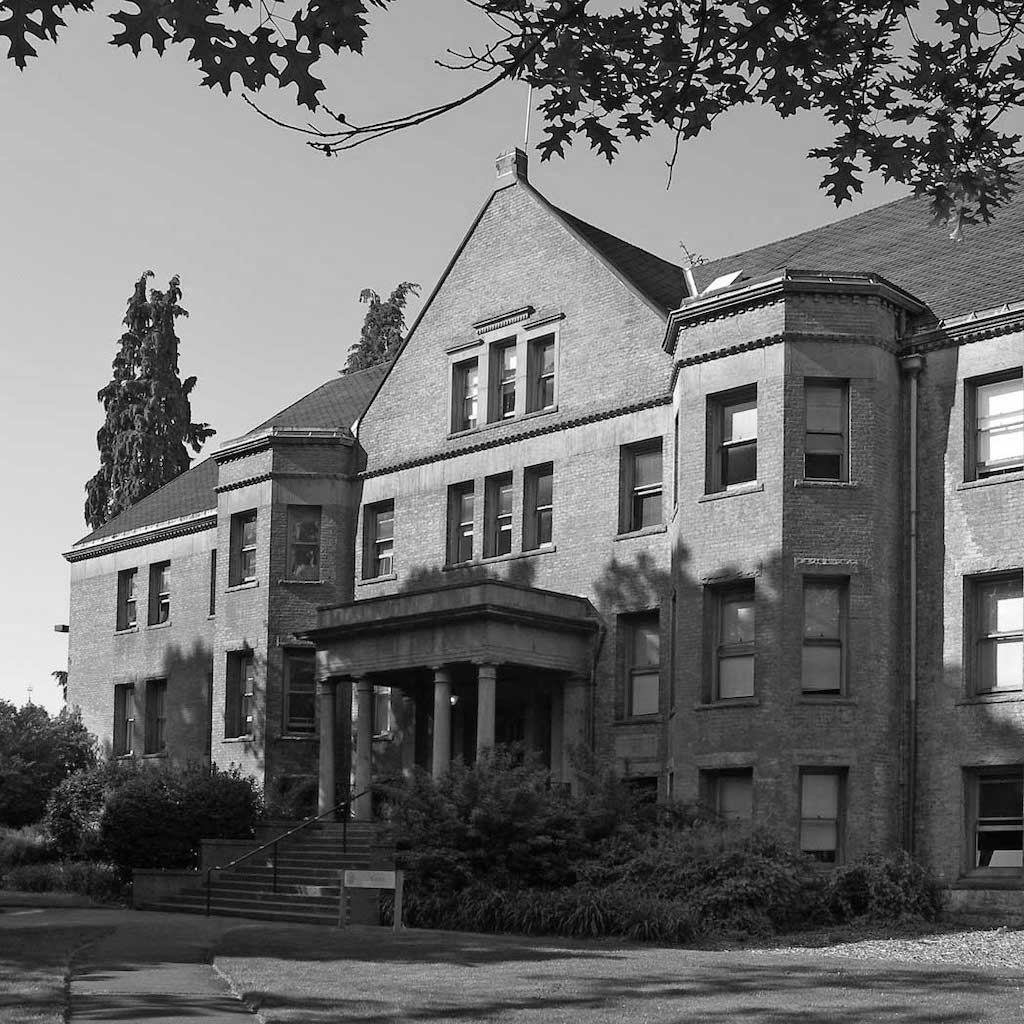
\includegraphics[width=0.4\textwidth]{images/lewis_grayscale_1024}
    \caption{\label{fig:lewis} A photo of Lewis -- the original signal $x^*$.}
\end{figure}
We use a greyscale 1024$\times$1024 photo of Lewis hall as the original signal (see figure \ref{fig:lewis}), and a random matrix $A \in \R^{2^{20}\times 2^{20}}$. As an initial point for algorithms we use the same photo with a certain percent of pixels missing. It allows us to vary the distance between the initial point and the solution and to analyze the algorithm's stability depending on its distance. However, this is a "sandbox" setting, as in a real-world we can not know a part of the solution to start with, one should use "Duchi initialization" process instead (see the Appendix A).

\lowtodo{Figure out what kind of data is available for academic phase retrieval.}

\section{Methods and Algorithm Design} % (fold)
\label{sec:methods}

\subsection{Algorithms} % (fold)
We adapt the Relax-and-Split algorithm for three different phase retrieval losses: the Algorithm \ref{alg:relax_and_split_for_first_loss} is from \cite{Zheng2018RelaxAndSplit}, but, to the best of our knowledge, there have been no adaptation of Relax-and-Split for \ref{eq:first_norm_and_square_phase_retrieval_loss}, and \ref{eq:double_square_phase_retrieval_loss}.

\label{sub:algorithms}
\subsection{Relax-and-Split for \ref{eq:first_norm_phase_retrieval_loss}} 
The Algorithm \ref{alg:relax_and_split_for_first_loss} is an adaptation of Algorithm \ref{alg:relax-and-split} for the \ref{eq:first_norm_phase_retrieval_loss} loss. To obtain it we relax this formulation as follows 

\eq{
    \label{eq:relaxed_first_loss}
    \min_{x \in \R^n,\, w \in \R^{kn}} \||w| - b\|_1 + \frac{1}{2\nu}\|Ax - w\|_2^2
}

The minimization over $x$ is a least-square procedure
\eq{
    x^{k+1} = (A^TA)^{-1}A^Tw^k = \frac{1}{k}A^Tw^k
}
where we used the fact that $A^TA = kI$. The minimization over $w$ is evaluation of a proximal operator 
\[
    w^{k+1} = \prox_{\nu\||\cdot|-b\|_1}(Ax^{k+1}) = ((|Ax^{k+1}| - b - \nu)_+ - (-|Ax^{k+1}|+b - \nu)_+ + b)_+
\]
see Lemma \ref{lemma:phase_retrieval_prox} for details. 

\begin{algorithm}
    \caption{Relax-and-Split for \ref{eq:first_norm_phase_retrieval_loss} (\cite{Zheng2018RelaxAndSplit}) }
    \label{alg:relax_and_split_for_first_loss}
    \begin{algorithmic}[1]
        \While{$\|x^{k+1} - x^k\| \geq \texttt{tol}$}
            \State $x^{k+1} \gets \frac{1}{k}A^Tw^{k}$ 
            \State $w^{k+1} \gets \prox_{\nu\||\cdot| - b\|}\pa{Ax}$ 
            \State $k \gets k+1$
        \EndWhile
        \Return $A^Tw^{k+1}$
    \end{algorithmic}
\end{algorithm}

\subsection{Relax-and-Split for \ref{eq:first_norm_and_square_phase_retrieval_loss}}
See Algorithm \ref{alg:relax_and_split_for_second_loss} for pseudocode. To obtain the adaptation which is compatible with Relax-and-Split we relax the objective \ref{eq:first_norm_and_square_phase_retrieval_loss} two times, which gives us

\eq{
    \label{eq:relaxed_semiquadratic_loss}
    \min_{x, w, z} \|z - b^2\|_1 + \frac{1}{2\nu}\|w - Ax\|^2 + \frac{1}{2\lambda}\|w^2 - z\|^2
}

The minimization over $x$ is, again, a least-square procedure 
\[
    x^{k+1} = \frac{1}{k}A^Tw^k
\]

For minimizing over $w$ we note that the loss \ref{eq:relaxed_semiquadratic_loss} is separable, so we can analyze $w_i^{k+1}$ separately

\begin{equation}
    \label{eq:w_subproblem}
    w^{k+1}_i = \argmin_{w} \frac{1}{2\nu}(w - a_i^Tx^{k+1})^2 + \frac{1}{2\lambda}\|w^2 - z^{k}_i\|^2
\end{equation}

One may think of it as of a proximal step:
\[
    w_i^{k+1} = \prox_{\frac{\nu}{\lambda}\|*^2 - z_i^k\|^2}(a^T_ix^{k+1})
\]

Plugging in coefficients for $w$ we get

\[
    \argmin_w \frac{1}{2\lambda}w^4 - \pa{\frac{z_i^{k}}{\lambda} - \frac{1}{2\nu}}w^2 - \frac{a_i^Tx^{k+1}}{\nu}w + \pa{\frac{(z_i^{k})^2}{2\lambda} + \frac{(a_i^Tx^{k+1})^2}{2\nu}}
\]

We have a fourth-order polynomial w.r.t. $w$ with positive higher-order coefficient $\frac{1}{2\nu}$, which means that the is a minimum in one of (at most) three possible roots, which have closed-form formulations. After taking a derivative we get

\eq{
    \label{eq:loss_2_roots_poly}
    w^3 - \pa{z_i^{k} - \frac{\lambda}{2\nu}}w - \frac{\lambda}{2\nu}a_i^Tx^{k+1} := w^3 - b_iw - c_i = 0
}

which roots, thanks to Wolfram, are listed in the Figure \ref{fig:roots}.

\begin{figure}[h!]
    \centering
    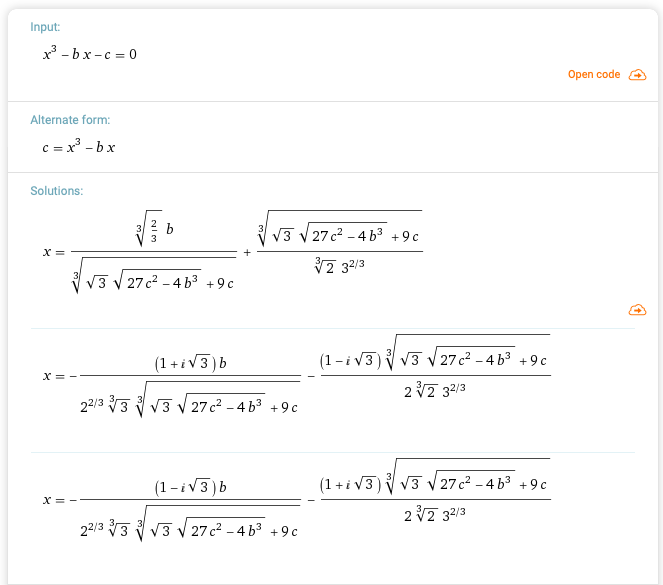
\includegraphics[width=0.7\textwidth]{images/roots}
    \caption{\label{fig:roots} Roots of a 3rd order polynomial, which are used in Algorithm \ref{alg:relax_and_split_for_second_loss}}
\end{figure}

These roots give us a closed form solution for the subproblem \ref{eq:w_subproblem}. 

For $z^{k+1}$ we have the same optimization subproblem as for $w$ in Algorithm \ref{alg:relax_and_split_for_first_loss}.

Putting all pieces together, we get Algorithm \ref{alg:relax_and_split_for_second_loss}.

\begin{algorithm}
    \caption{Relax-and-Split for \ref{eq:first_norm_and_square_phase_retrieval_loss}}
    \label{alg:relax_and_split_for_second_loss}
    \begin{algorithmic}[1]
        \While{$\|x^{k+1} - x^k\| \geq \texttt{tol}$}
            \State $x^{k+1} \gets \frac{1}{k}A^Tw^{k}$ 
            \State $w^{k+1}_i \gets \argmin_{w_1, w_2, w_3} \frac{1}{2\lambda}w^4 - \pa{\frac{z_i^{k}}{\lambda} - \frac{1}{2\nu}}w^2 - \frac{y_i}{\nu}w + \pa{\frac{(z_i^{k})^2}{2\lambda} + \frac{(a_i^Tx^{k+1})^2}{2\nu}},\ w_1, w_2, w_3 \text{ are roots of \ref{eq:loss_2_roots_poly}}$
            \State $z^{k+1} \gets \prox_{\lambda\||\cdot| - b^2\|}\pa{(w^{k+1})^2}$ 
            \State $k \gets k+1$
        \EndWhile
        \Return $A^Tw^{k+1}$
    \end{algorithmic}
\end{algorithm}

\begin{tip}
\Lesha{6/5/2019} Note that $w^{k+1}$ in Algorithm \ref{alg:relax_and_split_for_second_loss} depends on $z^k$, not on $z^{k+1}$, so there is a lag between variables which may affect convergence. 
\lowtodo{Ask Sasha whether the lag in Algorithm \ref{alg:relax_and_split_for_second_loss} is ok.}
\end{tip}

\subsection{Relax-and-Split for \ref{eq:double_square_phase_retrieval_loss}}
It's enough to relax the loss \ref{eq:double_square_phase_retrieval_loss} only once to obtain 
    \[
        \min_{x, w} \|w^2 - b^2\|_2^2 + \frac{1}{2\lambda}\|Ax - w\|_2^2
    \]
    Note that this optimization problem is exactly a subproblem from the Algorithm \ref{alg:relax_and_split_for_second_loss} with $x$ and $w$, and with the fixed $z^k := b^2$. 
    
\begin{algorithm}
    \caption{Relax-and-Split for \ref{eq:double_square_phase_retrieval_loss}}
    \label{alg:relax_and_split_for_thrird_loss}
    \begin{algorithmic}[1]
        \While{$\|x^{k+1} - x^k\| \geq \texttt{tol}$}
            \State $x^{k+1} \gets \frac{1}{k}A^Tw^{k}$ 
            \State $z_i^{k+1} = b^2$
            \State $w^{k+1}_i \gets \argmin_{w_1, w_2, w_3} \frac{1}{2\lambda}w^4 - \pa{\frac{z_i^{k}}{\lambda} - \frac{1}{2\nu}}w^2 - \frac{y_i}{\nu}w + \pa{\frac{(z_i^{k})^2}{2\lambda} + \frac{(a_i^Tx^{k+1})^2}{2\nu}},\ w_1, w_2, w_3 \text{ are roots of \ref{eq:loss_2_roots_poly}}$
            \State $k \gets k+1$
        \EndWhile
        \Return $A^Tw^{k+1}$
    \end{algorithmic}
\end{algorithm}

\section{Results} % (fold)

\begin{figure}
    \centering
    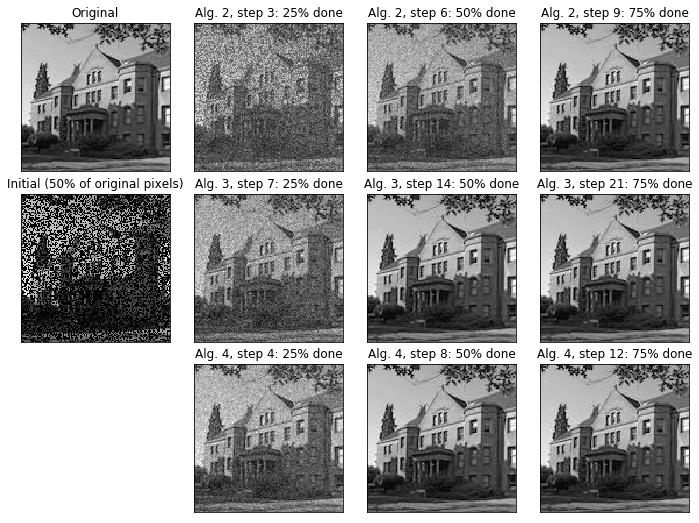
\includegraphics[width=\textwidth]{images/lewis_reconstruction}    
    \caption{\label{fig:lewis_reconstruction} A sample experiment on phase retrieval, when 50\% of original pixels are available.}
\end{figure}


The image reconstruction process for all three algorithms is displayed on the Figure

\label{sec:results}
Two experiments on the stability and performance of the algorithms \ref{alg:relax_and_split_for_first_loss}, \ref{alg:relax_and_split_for_second_loss}, and \ref{alg:relax_and_split_for_thrird_loss} were conducted.

\subsection{Sensitivity to Initial Guess}
\begin{figure}
    \centering
    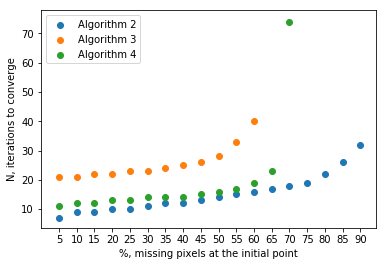
\includegraphics[width=0.5\textwidth]{images/results_initial_conds}
    \caption{\label{fig:resits_init_conds} Algorithms 3 and 4 are sensitive to the initial guess's quality: they stop converging after 60\% and 70\% are missing respectively. The same time, Algorithm 2 is more robust: successfully reconstructs the signal even when only 5\% of the original pixels are available.}
\end{figure}
\paragraph{Experimental setup} We fix the parameters of the algorithms as follows: $\lambda = 5000$, $\nu = 20$, the maximum number of iterations is $maxIter = 400$, the stopping criteria is $\|x^{k+1} - x^{k}\|^2 \leq tol = 10^{-3}$. We then sequentially initialize $x_0$ as $x^*$ with the given percent of missing pixels (x-axis) and count the number of iterations before convergence (y-axis), see the Figure \ref{fig:resits_init_conds}. If $maxIter$ iterations is made and the loss-function value is more than $10^{-5}$, then we consider this case to be divergent. The divergent cases are not displayed on the plot, so if a point is missing it means that the algorithm does not converge.
\paragraph{Experimental results}
The experiment shows (Figure \ref{fig:resits_init_conds}) that Algorithm \ref{alg:relax_and_split_for_first_loss} convergence even from the very distant initial points (95\% of pixels are missing), while Algorithms \ref{alg:relax_and_split_for_second_loss} and \ref{alg:relax_and_split_for_thrird_loss} are more sensitive to the quality of the initial guess: they stop converging when more than $70\%$ of pixels are missing.


\subsection{Sensitivity to Number of Measurements}
\begin{figure}[h!]
    \centering
    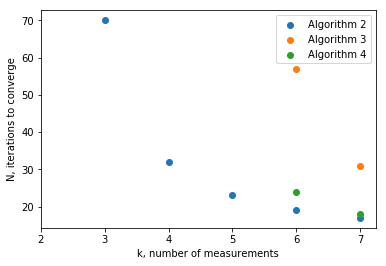
\includegraphics[width=0.5\textwidth]{images/result_number_of_measurements}
    \caption{\label{fig:resits_number_of_measurements} how many measurements of the signal do algorithms need for successful reconstruction when the initial guess contains only 5\% of the original pixels. We see that Algorithm 2 successfully finishes when 3 measurements are available, whereas Algorithms 3 and 4 require at least 6 measurements for successful reconstruction.}
\end{figure}
\paragraph{Experimental setup} We fix the parameters of the algorithms as follows: $\lambda = 5000$, $\nu = 20$, the maximum number of iterations is $maxIter = 400$, the stopping criteria is $\|x^{k+1} - x^{k}\|^2 \leq tol = 10^{-3}$, $x_0$ is $x^*$ with 95\% of pixels missing. We then sequentially initialize the problem with different number of measurements $k$ (x-axis), hence with different matrices A, and count the number of iterations before convergence (y-axis), see the Figure \ref{fig:resits_number_of_measurements}. If $maxIter$ iterations is made and the loss-function value is more than $10^{-5}$, then we consider this case to be divergent. The divergent cases are not displayed on the plot, so if a point is missing it means that the algorithm does not converge.
\paragraph{Experimental results}
 The second experiment (Figure \ref{fig:resits_number_of_measurements}) shows that Algorithm \ref{alg:relax_and_split_for_first_loss} works better when the number of measurements is small. In particular, Algorithm \ref{alg:relax_and_split_for_first_loss} required three measurements of the signal to recover the image having $5\%$ of original pixels at the initial point, while Algorithms \ref{alg:relax_and_split_for_second_loss} and \ref{alg:relax_and_split_for_thrird_loss} required at least 6 measurements to converge from the same initial guess. 

\section{Conclusion}
    We showed that solving the exact original formulation of academic phase retrieval problem (eq. \ref{eq:first_norm_phase_retrieval_loss}) with Relax-and-Split method may be advantageous over solving quadratic relaxations of it (eq. \ref{eq:first_norm_and_square_phase_retrieval_loss} and \ref{eq:double_square_phase_retrieval_loss}). The non-smooth formulation, although seems harder to solve, provides more robust solution, is less sensitive to the initial guess, and requires less measurements of the signal for successful phase reconstruction.        

\appendix
\section{Proofs}
\begin{lemma} \textbf{(Prox for shifted absolute value)}
    \label{lemma:phase_retrieval_prox}
    Let $h$ to be defined as
    \[
        h(x) = ||x|-b|, \ b \in \R_+ 
    \]
    then the proximal operator of $h$ is 
    \[
        \prox_{\nu h}(y) = \pa{\pa{|y| - b - \nu}_+ - \pa{-|y| + b - \nu}_+ + b}_+
    \]
\end{lemma}
\begin{proof}
    By definition 
    \[
        \prox_{\nu h}(y) = \argmin_{x \in \R} \frac{1}{2\nu}(x - y)^2 + ||x|-b| = 
    \]
    \begin{tip}
    \Peng{6/3/19} This is equivalent to
    \lowtodo{It works, but I still don't understand why this transition is true. Ask Peng again.}
    \end{tip} 
    \[
        = \argmin_{|x| \in \R_+} \frac{1}{2\nu}(|x|-|y|)^2 + ||x| - b| = \argmin_{z \geq 0}\frac{1}{2\nu}(z - |y|)^2 + |z-b| = 
    \]
    which is just a $\prox$ of a shifted absolute value of the point $|y|$
    \[
        = \prox_{\nu|z-b|}(|y|)
    \]
    which is, according to \cite{Parikh2014} Eq. 2.2 (precomposition) and Eq. 6.9, is equal to
    \[
        = ((|y| - b - \nu)_+ - (-|y|+b - \nu)_+ + b)_+
    \]
    where the outer positive slice comes from the constraint $z \geq 0$.
    \begin{tip}
        \Peng{6/3/19} I forgot about this last slice and everything worked out anyway. 
        \lowtodo{Check that it really works both ways and figure out why.}    
    \end{tip}

\end{proof}

\subsection*{''Duchi Inicialization''} We initialize $x_0$ with ''Duchi Inicialization'' (Algorithm 2 from \cite{Duchi2017PhaseRetrival}).

\begin{tip}
    \Lesha{6/5/19} \textit{This part is postponed}, because by now \ref{eq:first_norm_phase_retrieval_loss} with relax-and-split converges from pretty distant initial points (like, when 95\% pixels are missing). Need more motivation to consider such a cumbersome initialization routine.
\end{tip}
 
 In particular, we make an estimation of the norm and the direction for a (global?) solution for the problem:

\eq{
    \label{eq:duchi_initialization}
    \hat{r}^2 & := \frac{1}{m}\sum_i b_i \\
    \mathcal{I} & := \bra{i: \ b_i \leq \half \hat{r}^2} \\
    X^{init} & := \sum_{i \in \mathcal{I}} a_ia_i^H \\
    \hat{d} & := \argmin_{d \in \unitsphere{0}}d^TX^{init}d \\
    \hat{x} & := \hat{d}\hat{r}
} 

\hightodo{It looks like $\hat{r}^2 = \frac{1}{m}\sum_i b_i^2$ in case of \ref{eq:first_norm_phase_retrieval_loss} and as stated above for \ref{eq:first_norm_and_square_phase_retrieval_loss} and \ref{eq:double_square_phase_retrieval_loss}. Check it out.}

We do not have an access to columns and rows of $A$, so we can't explicitly compose $X^{init}$. Yet we can work with it implicitly: 
\[
    X^{init}y = A^T(\mathcal{I}\odot Ay)
\]
Where by $\odot$ we mean an element-vise (Hadamard) product. 
Clearly, we're looking for the eigenvector which corresponds to the minimal eigenvalue.
\begin{tip}
    \Peng{in \cite{Zheng2018RelaxAndSplit}} we use 10 power iterations for initialization.
    \hightodo{Power initialization looks for $\lambda_{max}$, which means we maximize the optimization subproblem instead of minimization. Ask Peng.}
\end{tip}

\section{Resources}

%----------------------------------------------------------------------------------------
%   REFERENCE LIST
%----------------------------------------------------------------------------------------
\bibliographystyle{alpha}
\bibliography{phase_retrieval_bibliography}
\clearpage

\end{document}